\chapter{Introducción}
\pagenumbering{arabic}

\section{Motivación}

La Inteligencia Artificial (IA) gana cada año mas popularidad, como se muestra en la Figura \ref{fig:ai_grow}.

% Vertically alling two sufigures and keep subcaption using floatrow and subcaptions pkgs
\begin{figure}[htb]
  \floatsetup{heightadjust=all, valign=c}
  \begin{subcaptiongroup}
  \begin{floatrow}
    \ffigbox{%
      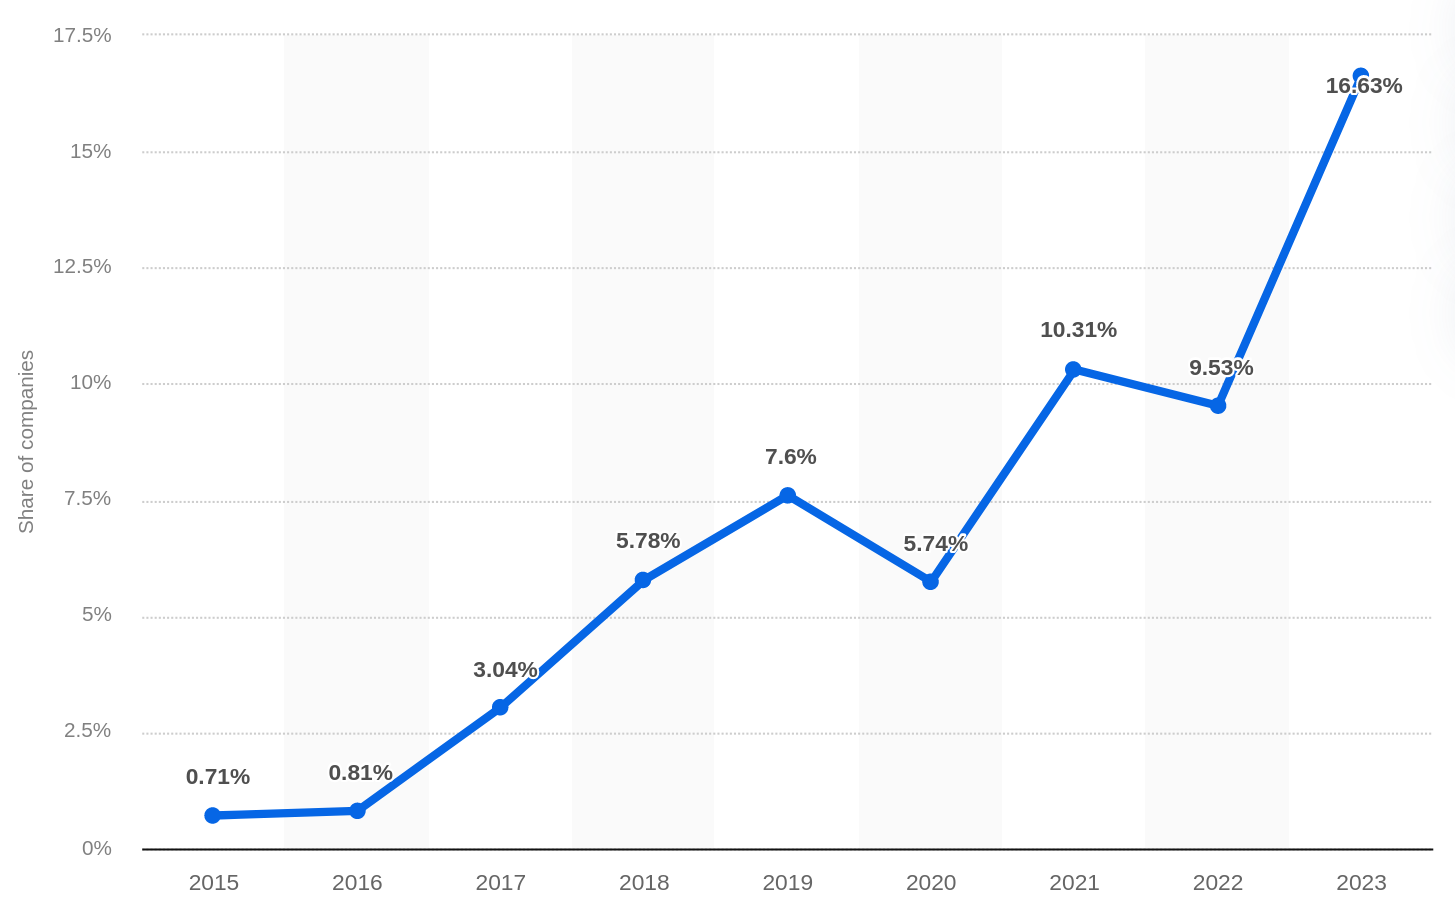
\includegraphics[width=0.48\textwidth]{root/Imagenes/1_intro/ai_interest.png}
    }{%
      \caption{Interés de las empresas \cite{ai_interest_growth}.}%
    }
    \ffigbox{%
      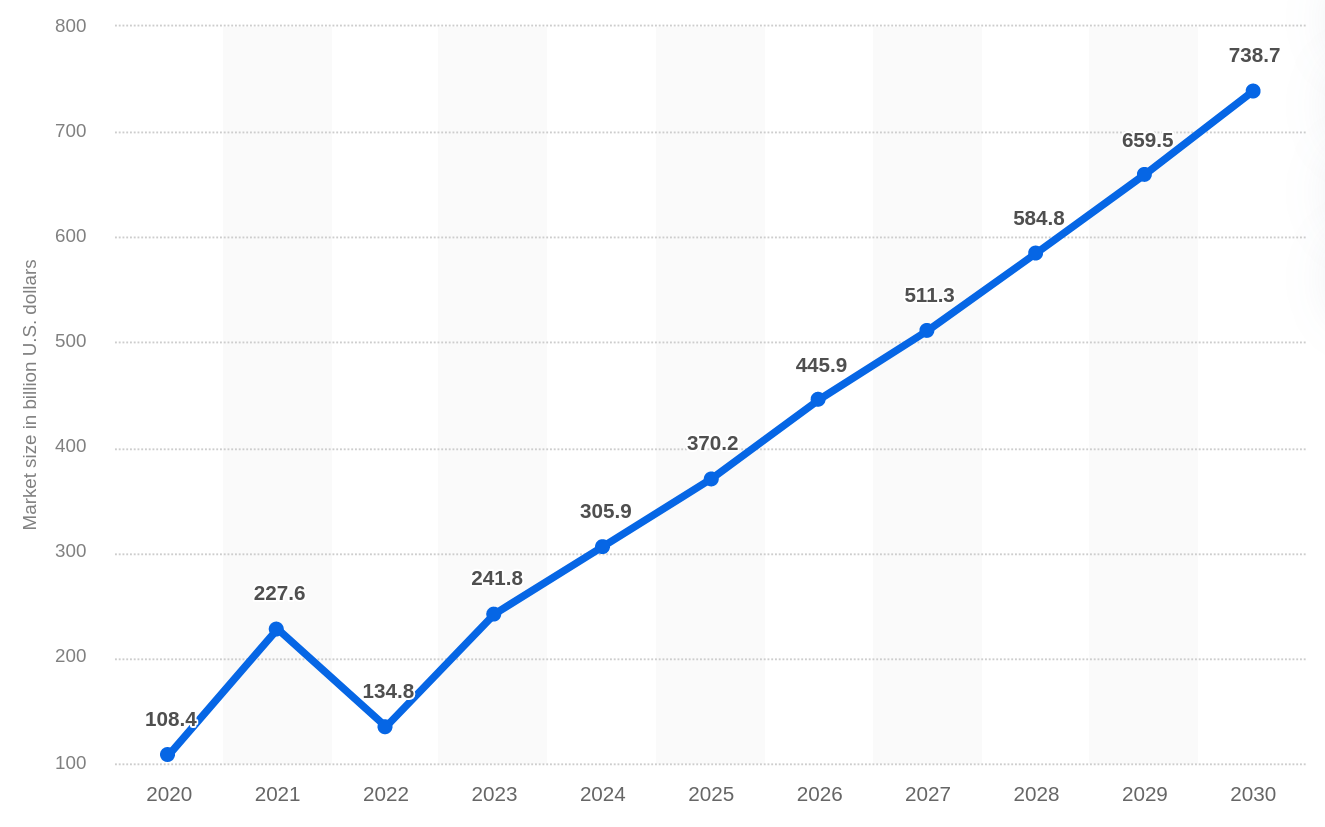
\includegraphics[width=0.49\textwidth]{root/Imagenes/1_intro/market_size.png}
    }{%
      \caption{Valor de mercado \cite{ai_market_size}.}%
    }
  \end{floatrow}
  \end{subcaptiongroup}
  \caption{Crecimiento de la IA en los últimos 10 años y crecimiento esperado.}%
  \label{fig:ai_grow}%
\end{figure}

Al aumentar este interés y por tanto su uso en diversos campos también lo hará el consumo energético. La motivación principal de este trabajo es desarrollar componentes hardware para aumentar la eficiencia energética de algoritmos de IA. Concretamente este trabajo se centra el en un tipo de redes neuronales (\textit{\textbf{N}eural \textbf{N}etwork}) llamadas redes neuronales bayesianas (\textit{\textbf{B}ayesian \textbf{N}eural \textbf{N}etwork}). Estas redes permiten calcular la incertidumbre de sus predicciones lo que aporta transparencia en su uso. En relación, otra de las motivaciones de este trabajo es fomentar el uso de este tipo de redes para, en consecuencia, fomentar el uso de IA transparente, siguiendo la filosofía de la Ley de Inteligencia Artificial de la Unión Europea \cite{eu_ai}. Otra de las motivaciones principales de este trabajo es fomentar el desarrollo de la arquitectura RISC-V, también en concordancia con otro proyecto europeo, el \textit{European Processor Initiative} (EPI) \cite{european_processor}.

Concretamente este trabajo se centra en la combinación de la IA, concretamente el aprendizaje automático  (\textbf{M}achine \textbf{L}earning), y el internet de las cosas (\textit{\textbf{I}nternet \textbf{o}f \textbf{T}hings}). Esta combinación se conoce comúnmente como TinyML y tiene un gran potencial a la hora de reducir el consumo energético \cite{tinyML_sustainable}. Los componentes IoT son mas eficientes energéticamente que los procesadores de altas prestaciones, por lo que trasladar la ejecución de los algoritmos de IA a estos componentes reduciría su consumo además de eliminar comunicaciones costosas entre componentes IoT desplegados y servidores.

\section{Objetivos y alcance}

El objetivo principal de este trabajo es optimizar la inferencia de BNN en un procesador RISC-V de bajas prestaciones. Se han seguido los siguientes pasos para lograr el objetivo:
\begin{enumerate}
    \item Estudiar el funcionamiento de la inferencia de las BNN.
    \item Analizar aceleradores existentes de inferencia de BNN.
    \item Investigar el soporte existente para ejecutar inferencia de BNN en procesadores de bajas prestaciones sin precisión de punto flotante.
    \item Implementar una librería en C junto a herramientas que permitan ejecutar la inferencia de BNN en un procesador RISC-V desarrollado en un trabajo previo \cite{riscv_tfg}.
    \item Validar la librería implementada con diferentes modelos.
    \item Analizar la carga de trabajo de la librería desarrollada.
    \item Desarrollar optimizaciones software y analizar sus ventajas y desventajas.
    \item Investigar sobre generadores de números aleatorios gaussianos (\textit{\textbf{G}aussian \textbf{R}andom \textbf{N}umber \textbf{G}enerator}).
    \item Diseñar un GRNG que se pueda integrar en el procesador RISC-V como una extensión.
    \item Estudiar los pasos necesarios para extender un procesador RISC-V y poder utilizar la extensión desde código en alto nivel C.
    \item Analizar el coste y rendimiento de la extensión utilizando una (\textit{\textbf{F}ield \textbf{P}rogrammable \textbf{G}ate \textbf{A}rray}).
\end{enumerate}

Todo el código de este trabajo se encuentra disponible en un repositorio público en GitHub \cite{bnn_github}.

%% quizas aqui se puede poner que lo hemos enviado al congreso y las JJI

\section{Herramientas Utilizadas}

El diseño del procesador base se encuentra en el repositorio riscv-vhdl \cite{base_riscv_cpu_git}. Para definir la extensión del procesador RISC-V se ha utilizado el lenguaje de especificación hardware VHDL. Para simular el comportamiento del procesador se ha utilizado el simulador GHDL \cite{ghdl} junto con el visor de ondas GTKWave \cite{gtkwave}. Para compilar programas en C para el procesador se ha utilizado el conjunto de herramientas GNU RISC-V Compiler Toolchain \cite{gcc_riscv}. 

Para entrenar BNNs se ha utilizado la biblioteca de Python TensorFlow Probability \cite{tfprob} junto al repositorio BNN\_for\_hyperspectral\_datasets\_analysis \cite{bnn_hyper_git}. El proceso de compilación y pruebas se han automatizado todo lo posible mediante la herramienta Make y \textit{scripts} en Bash y Python. Para manejar ficheros ELF desde Python se ha utilizado la biblioteca pyelftools \cite{pyelftools}. Para crear gráficas se ha utilizado la biblioteca de Python Matplotlib \cite{matplotlib}. Como programa de control de versiones se ha utilizado Git \cite{git} junto con GitHub como repositorio en línea.

Se ha utilizado la plataforma de desarrollo Xilinx ZCU104 FPGA \cite{fpga_board} junto a Vivado Design Suite \cite{vivado} para implementar los diseños hardware sobre una FPGA y analizar sus costes.

Para redactar este documento se ha utilizado el editor de \LaTeX\ en línea Overleaf \cite{overleaf} y para crear los diagramas se utilizado el editor en línea draw.io \cite{drawio} junto al editor de gráficos vectoriales Inkscape.
